\documentclass[a4paper]{arrowhead}

\usepackage[yyyymmdd]{datetime}
\usepackage{etoolbox}
\usepackage[utf8]{inputenc}
\usepackage{multirow}

\renewcommand{\dateseparator}{-}

%% Special references
\newcommand{\scref}[2]{{\textcolor{ArrowheadBlue}{\hyperref[sec:services:consumed:#1]{#2}}}}
\newcommand{\scdef}[2]{{\textcolor{ArrowheadBlue}{#2\label{sec:services:consumed:#1}}}}
\newcommand{\spref}[2]{{\textcolor{ArrowheadBlue}{\hyperref[sec:services:produced:#1]{#2}}}}
\newcommand{\spdef}[2]{{\textcolor{ArrowheadBlue}{#2\label{sec:services:produced:#1}}}}
%%

\begin{document}

%% Arrowhead Document Properties
\ArrowheadTitle{Orchestrator}
\ArrowheadType{System Design Description}
\ArrowheadTypeShort{SysDD}
\ArrowheadVersion{4.3.0}
\ArrowheadDate{\today}
\ArrowheadAuthor{Szvetlin Tanyi}
\ArrowheadStatus{RELEASE}
\ArrowheadContact{szvetlin@aitia.ai}
\ArrowheadFooter{\href{www.arrowhead.eu}{www.arrowhead.eu}}
\ArrowheadSetup
%%

%% Front Page
\begin{center}
  \vspace*{1cm}
  \huge{\arrowtitle}

  \vspace*{0.2cm}
  \LARGE{\arrowtype}
  \vspace*{1cm}
  \vspace*{\fill}

  % Front Page Image
  %\includegraphics{figures/TODO}

  \vspace*{1cm}
  \vspace*{\fill}

  % Front Page Abstract
  \begin{abstract}
    This document describes the Orchestrator core system of the Eclipse Arrowhead Framework. The Orchestrator provides runtime (late) binding between Application Systems.
  \end{abstract}

  \vspace*{1cm}

  \scriptsize
  \begin{tabularx}{\textwidth}{l X}
    \raisebox{-0.5\height}{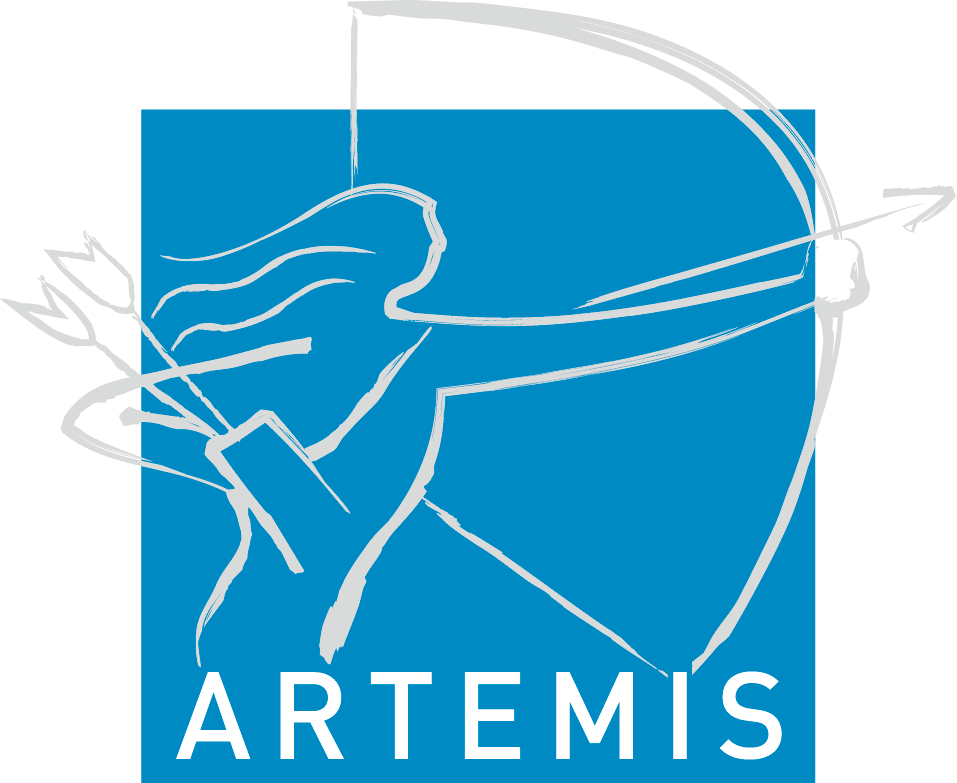
\includegraphics[width=2cm]{figures/artemis_logo}} & {ARTEMIS Innovation Pilot Project: Arrowhead\newline
    THEME [SP1-JTI-ARTEMIS-2012-AIPP4 SP1-JTI-ARTEMIS-2012-AIPP6]\newline
    [Production and Energy System Automation Intelligent-Built environment and urban infrastructure for sustainable and friendly cities]}
  \end{tabularx}
  \vspace*{-0.2cm}
\end{center}
\newpage
%%

%% Table of Contents
\tableofcontents
\newpage
%%

\section{Overview}
\label{sec:overview}

This document describes the Eclipse Arrowhead Orchestrator system. 
The primary purpose for the Orchestrator System is to provide Application Systems with orchestration information: where they need to connect to. The outcome of the "Orchestration Service" include rules that will tell the Application System what Service provider System(s) it should connect to and how (acting as a Service Consumer). Such orchestration rules include:

\begin{itemize}
    \item Accessibility information details of a Service provider (e.g network address and port)
    \item Details of the Service instance within the provider System (e.g. base URL, IDD specification and other metadata)
    \item Authorization-related information (e.g. access token and signature)
    \item Additional information that is necessary for establishing connection
\end{itemize}

This orchestration rule information can reach the given Application System (consumer) in two different ways: the System itself can request it ("pull") or the Orchestrator itself can update the System when it is needed ("push method"). However, in both cases, there shall be an underlying, hidden process ("orchestration process"), which ensures the consistence of state between the various Core Systems.

In G4.0, only the pull method is implemented and the Orchestrator shall negotiate with the other Core Systems while trying to facilitate the new service request (or trying to push a new status). This is necessary for the following cases and requirements (basically, when ad hoc, unsupervised connections are not allowed):

\begin{itemize}
    \item When accountability is required for all Systems in the Local Cloud: connections cannot be established without the knowledge, approval and logged orchestration events of the Core Systems ("central governance").
    \item QoS and resource management reasons: ad hoc peer-to-peer connections cannot be allowed in certain managed networks and deployment scenarios. Every connection attempt shall be properly authorized and its QoS expectations (resource reservations) handled.
    \item Inter-Cloud orchestration can only happen via negotiations between the two Core System sets. Ad hoc inter-cloud connections shall not be allowed in the Arrowhead framework.
\end{itemize}

In these cases, when the Orchestrator is the sole entry point to establishing new connections within the Local Cloud, Application Systems do not have the possibility to skip any of the control loops with all the appropriate Core Systems. When such security and safety concerns are not present, the orchestration process might be cut back or these interactions between Core Systems might be limited. Within G4.0, this is not the primary use case, but it is allowed. With the proper self-implemented (modified) and a self-compiled Orchestrator can fit the deployment best.

Therefore, the Orchestrator provides two core Services and may consume many other ones, but at least two -- again, depending on its deployment. This figure depicts the mandatory and optional interfaces of this System.

This System (in line with all core Systems) utilizes the X.509 certificate Common Name naming convention in order to work.
The v4.3.0 only supports the HTTP protocol, JSON encoding and TLS payload protection. 


\section{System Role}
\label{sec:role}

This System only provides two Core Service the \textbf{Orchestration} and \textbf{OrchestrationStoreManagement}. 

The Orchestrator mainly consumes services from other Core Systems in order to fulfil its primary functionality: provide connection targets for Application Systems in a secure and resource managed manner -- hence build an SoS.

During this orchestration process the Orchestrator either facilitates a service request from an Application System or processes a system-of-systems (SoS) level choreography push from the Plant Description Engine ("Choreographer"). For the latter case, the Orchestrator System consumes the OrchestrationPush from affected Application Systems in order to deliver a renewed set of connection rules to them.

Within the Orchestrator, there is a database which captures design time bindings between Application Systems, the Orchestration Store. Operators of the Cloud and other System-of-Systems designer tools ("SoS Choreographers") are allowed to modify the rules stored in the Orchestration Store, other generic Application Systems are not.

The ServiceDiscovery Service is used to publish the Orchestration Service in the Service Registry. This Service is also used to query the Service Registry and fetch (metadata) information on other Application Systems.

The Services of the Authorization System can be used to verify access control and implement other security-related administration tasks.

The Services of the Gatekeeper can be utilized when inter-Cloud collaboration, servicing is required.

The Services of the QoS management System can be used to manage device, network and service-level Quality of Service agreements and configurations.

Orchestrator can be used in two ways. The first one uses predefined rules (coming from the Orchestrator Store DB) to find the appropriate providers for the consumer. The second option is the dynamic orchestration in which case the core service searches the whole local cloud (and maybe some other clouds) to find matching providers.

\section{Services}
\label{sec:services}

Meanwhile the consumed Services can vary, depending on the instantiation/installation of this System. 
\subsection{Consumed Services}

\subsubsection{\spdef{ServiceDiscovery}{ServiceDiscovery}}

This service is provided to allow other systems to \textbf{Register}
and to \textbf{Unregister} their services, and to \textbf{Query}
public services. In addition the service can Echo that its alive.

\subsubsection{\spdef{AuthorizationControl}{AuthorizationControl}}

This service is provided to allow the Orchestrator to check whether the requester is allowed to access the requested service..

\subsubsection{\spdef{TokenGeneration}{TokenGeneration}}

This service is provided to allow access token generation for a consumer system.

\subsubsection{\spdef{GlobalServiceDiscovery}{GlobalServiceDiscovery}}

This service enables service discovery between neighboring clouds.

\subsubsection{\spdef{Inter-CloudNegotiations}{Inter-CloudNegotiations}}

This service allows inter cloud connections to be negotiated.

\subsubsection{\spdef{QoSVerify}{QoSVerify}}

This service enables verification of the connection between systems.

\subsubsection{\spdef{QoSReserve}{QoSReserve}}

This service enables reserving a specified QoS level connection between systems

\subsection{Provided Services}

\subsubsection{\spdef{Orchestration}{Orchestration}}

This service is provided to allow the Orchestrator to check whether the requester is allowed to access the requested service. 

\subsubsection{\spdef{OrchestrationStoreManagement}{OrchestrationStoreManagement}}

This service is provided to allow access token generation for a consumer system.

\section{Security}
\label{sec:security}

This System can be secured via the HTTPS protocol. If it is started in secure mode, it verifies whether the Application System possesses a proper X.509 identity certificate and whether that certificate is Arrowhead compliant in its' making. This certificate structure and creation guidelines ensure:

\begin{itemize}
    \item Application System is properly bootstrapped into the Local Cloud
    \item The Application System indeed belongs to this Local Cloud
    \item The Application System then automatically has the right to register its Services in the Registry.
   
\end{itemize}

 If these criteria are met, the Application System’s registration or removal message is processed. An Application System can only delete or alter entries that contain the Application System as the Service Provider in the entry.

\newpage

\bibliographystyle{IEEEtran}
\bibliography{bibliography}

\newpage

\section{Revision History}
\subsection{Amendments}

\noindent\begin{tabularx}{\textwidth}{| p{1cm} | p{3cm} | p{2cm} | X | p{4cm} |} \hline
\rowcolor{gray!33} No. & Date & Version & Subject of Amendments & Author \\ \hline

1 & 2020-12-05 & 4.3.0 &  & Tanyi Szvetlin \\ \hline


\end{tabularx}

\subsection{Quality Assurance}

\noindent\begin{tabularx}{\textwidth}{| p{1cm} | p{3cm} | p{2cm} | X |} \hline
\rowcolor{gray!33} No. & Date & Version & Approved by \\ \hline

1 & 2021-01-26 & 4.3.0 & Jerker Delsing \\ \hline

\end{tabularx}

\end{document}